\chapter{网页设计}

\section{主页(index.html)的设计}

Html部分较为清晰简单,主页上部设计一列导航栏,主体部分分为左中右三个大部分,每个大部分分为两个小部分,后期将使用Echarts绘制图表并进行响应式布局。

\lstset{
 columns=fixed,       
 numbers=left,                                        % 在左侧显示行号
 numberstyle=\tiny\color{gray},                       % 设定行号格式
 frame=none,                                          % 不显示背景边框
 backgroundcolor=\color[RGB]{245,245,244},            % 设定背景颜色
 keywordstyle=\color[RGB]{40,40,255},                 % 设定关键字颜色
 numberstyle=\footnotesize\color{darkgray},           
 commentstyle=\it\color[RGB]{0,96,96},                % 设置代码注释的格式
 stringstyle=\rmfamily\slshape\color[RGB]{128,0,0},   % 设置字符串格式
 showstringspaces=false,                              % 不显示字符串中的空格
 language=html,                                        % 设置语言
}
\begin{lstlisting}
    <div class="row-cols-md-4 row">
        <div id="l1">我是左1</div>
        <div id="l2">我是左2</div>
    </div>
    <div class="row-cols-md-4 row">
        <div id="c1" class="row clearfix">
            <div class="txt"><h2 class="text-lg-center text-center">累计确诊</h2></div>
            <div class="txt"><h2 class="text-lg-center text-center">剩余疑似</h2></div>
            <div class="txt"><h2 class="text-lg-center text-center">累计治愈</h2></div>
            <div class="txt"><h2 class="text-lg-center text-center">累计死亡</h2></div>
            <div class="num"><h1 class="text-primary text-center"></h1></div>
            <div class="num"><h1 class="text-primary text-center"></h1></div>
            <div class="num"><h1 class="text-primary text-center"></h1></div>
            <div class="num"><h1 class="text-primary text-center"></h1></div>
        </div>
        <div id="c2">我是中2</div>
    </div>
    <div class="row-cols-md-4 row">
        <div id="r1">我是右1</div>
        <div id="r2">我是右2</div>
    </div>
\end{lstlisting}

\section{数据可视化}

为了使得该系统在不同屏幕尺寸的设备上能够正确显示,按照Bootstrap框架对前端网页进行构建。页面顶部为导航栏(navbar navbar-default),作为不同功能分区以及后续更多功能的入口,右端搜索接口接入百度搜索,提供更为丰富的搜索功能。页面主体分为三个大部分,其中包括六个小部分,并按从左到右排列,每个div的id依次记为l1,l2,c1,c2,r1,r2。对于每一个列,其div的class设置为row-cols-md-4 row,以实现响应式布局。左上角l1为全国累计趋势曲线表,使用ECharts库以实现绘制。因为纵轴所表示的两个数值差距过大,l1与l2使用两个y轴绘制,并使用不同颜色加以区分。

在utils.py中,定义了每个div获取数据的方法,例如getunderline{~}l1underline{~}data,通过调用utils.py中的方法,从而连接到数据库并获得每个div所需的数据data。在controller.js中定义了数据在图表中的显示形式。

\begin{figure}[H]
    \centering
    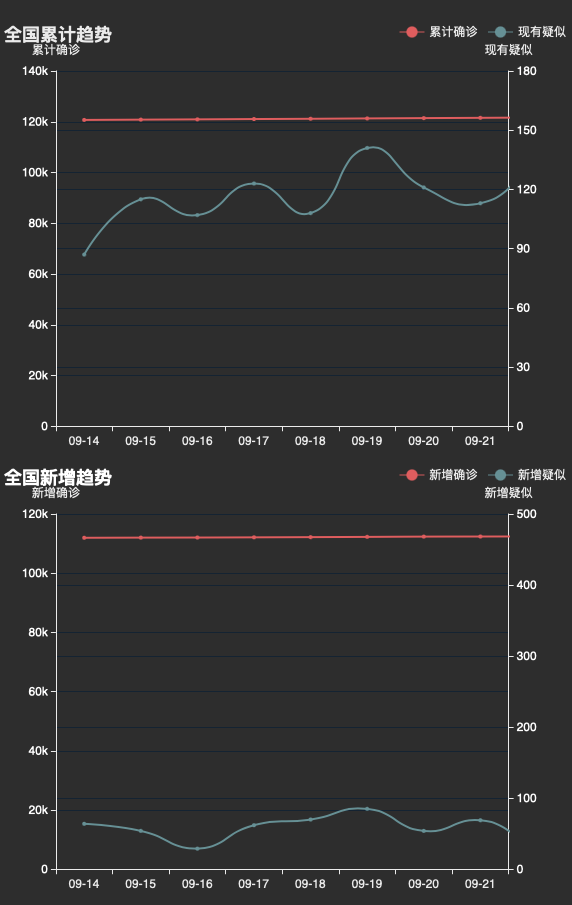
\includegraphics[width=0.8\textwidth]{t4}
    \bicaption{全国累计趋势与新增趋势}{National cumulative trends and new trends}
    \label{fig:t4}
\end{figure}

中上数据统计部分,使用类选择器显示当前累计确诊、剩余疑似、累计治愈以及累计死亡数据。

\lstset{
 columns=fixed,       
 numbers=left,                                        % 在左侧显示行号
 numberstyle=\tiny\color{gray},                       % 设定行号格式
 frame=none,                                          % 不显示背景边框
 backgroundcolor=\color[RGB]{245,245,244},            % 设定背景颜色
 keywordstyle=\color[RGB]{40,40,255},                 % 设定关键字颜色
 numberstyle=\footnotesize\color{darkgray},           
 commentstyle=\it\color[RGB]{0,96,96},                % 设置代码注释的格式
 stringstyle=\rmfamily\slshape\color[RGB]{128,0,0},   % 设置字符串格式
 showstringspaces=false,                              % 不显示字符串中的空格
 language=html,                                        % 设置语言
}
\begin{lstlisting}
    function get_c1_data() {
    $.ajax({
        url: "/c1",
        success: function (data) {
            $(".num h1").eq(0).text(data.confirm);
            console.log(data.confirm);
            $(".num h1").eq(1).text(data.suspect);
            $(".num h1").eq(2).text(data.heal);
            $(".num h1").eq(3).text(data.dead);
        },
        error: function (xhr, type, errorThrown) {

        }
    })
}
\end{lstlisting}


\section{对手机设备的适配}

为了使得该系统可以在手机设备上显示,在main.css中加入了旋转屏幕的样式。当屏幕尺寸判断为竖屏时,将旋转页面,使其变为横屏。

\begin{lstlisting}
    @media screen and (orientation: portrait) {
        html{
            width : 100vmin;
            height : 100vmax;
        }
        body{
            width : 100vmin;
            height : 100vmax;
        }
        #gyroContain{
            width : 100vmax;
            height : 100vmin;
            transform-origin: top left;
            transform: rotate(90deg) translate(0,-100vmin);
        }
      }
    @media screen and (orientation: landscape) {
        html{
            width : 100vmax;
            height : 100vmin;
        }
        body{
            width : 100vmax;
            height : 100vmin;
        }
        #gyroContain{
            width : 100vmax;
            height : 100vmin;
        }
    }
\end{lstlisting}






